\section*{Figures}

\begin{figure}[!ht]
\begin{subfigure}[t]{0.5\linewidth}
   \centering
   \caption{T4 lysozyme (L99A)}
   \label{fig:T4-L99A_protein}
   \frame{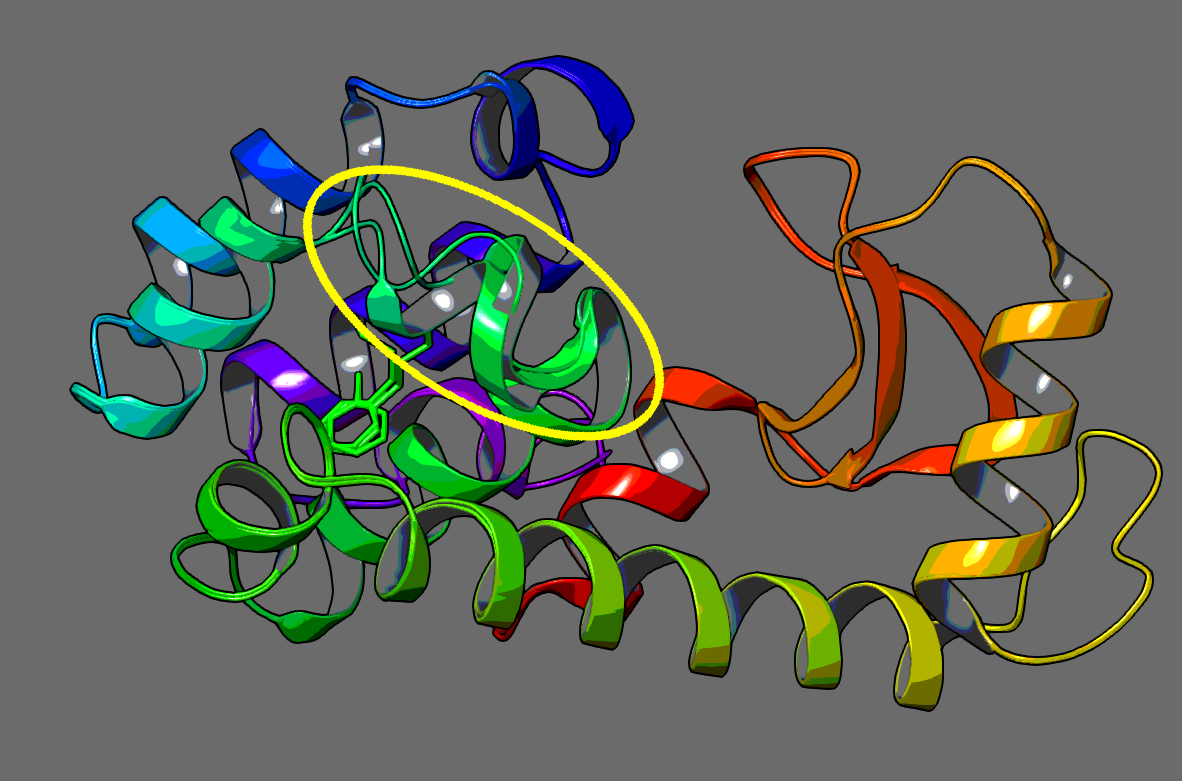
\includegraphics[clip, height=0.25\textheight, width=\linewidth]{Figures/Protein/T4_lysozyme_edit.png}}
\end{subfigure}\hfill
\centering
\begin{subfigure}[t]{0.5\linewidth}
  \centering
  \caption{F-helix (residues 107-115)}
  \label{fig:T4-L99A_tube}
  \frame{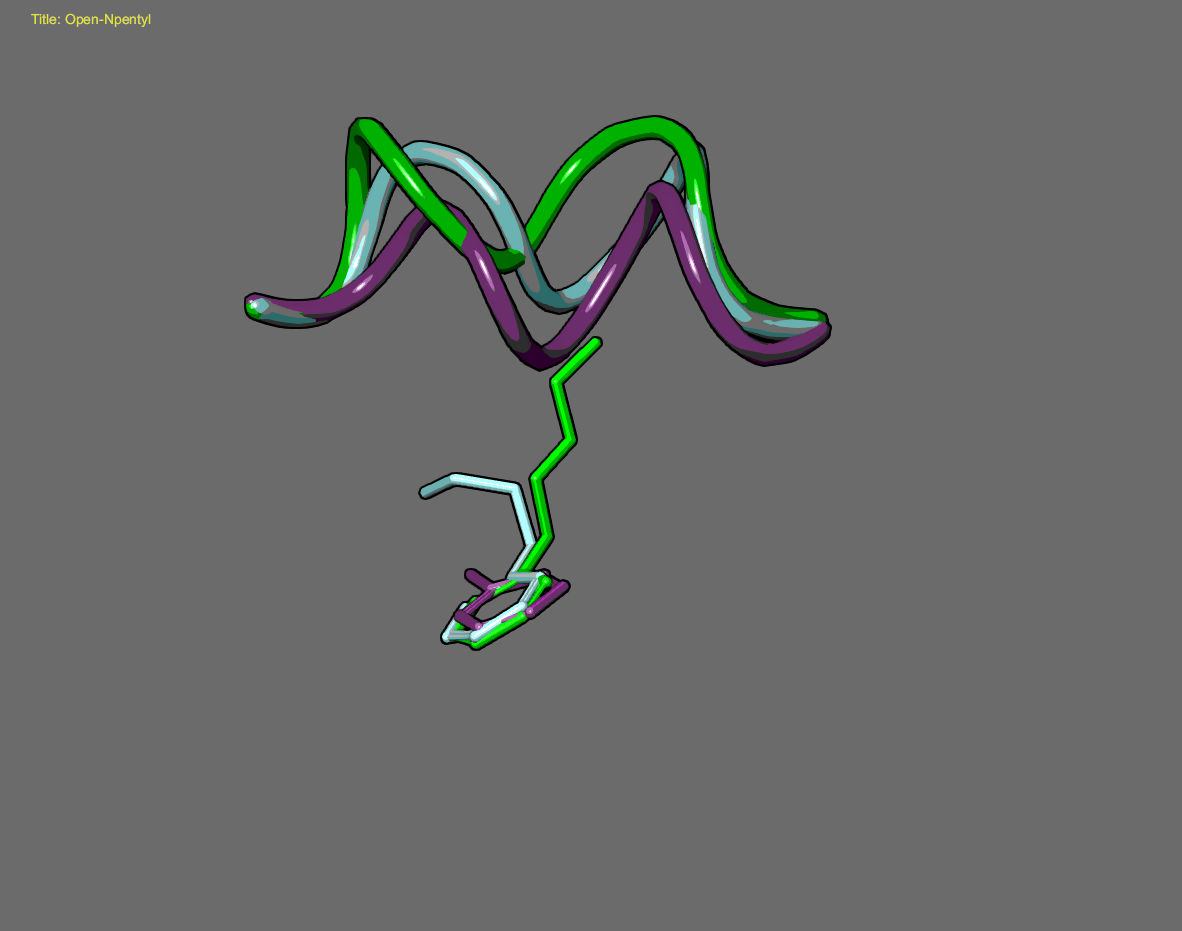
\includegraphics[trim={8cm 8cm 12cm 3cm}, clip, height=0.25\textheight, width=\linewidth]{Figures/Protein/ProteinTube.png}}
\end{subfigure}\hfill
\begin{subfigure}{0.30\textwidth}
   \centering
   \caption{Closed State}
   \label{fig:closed_surface}
   \frame{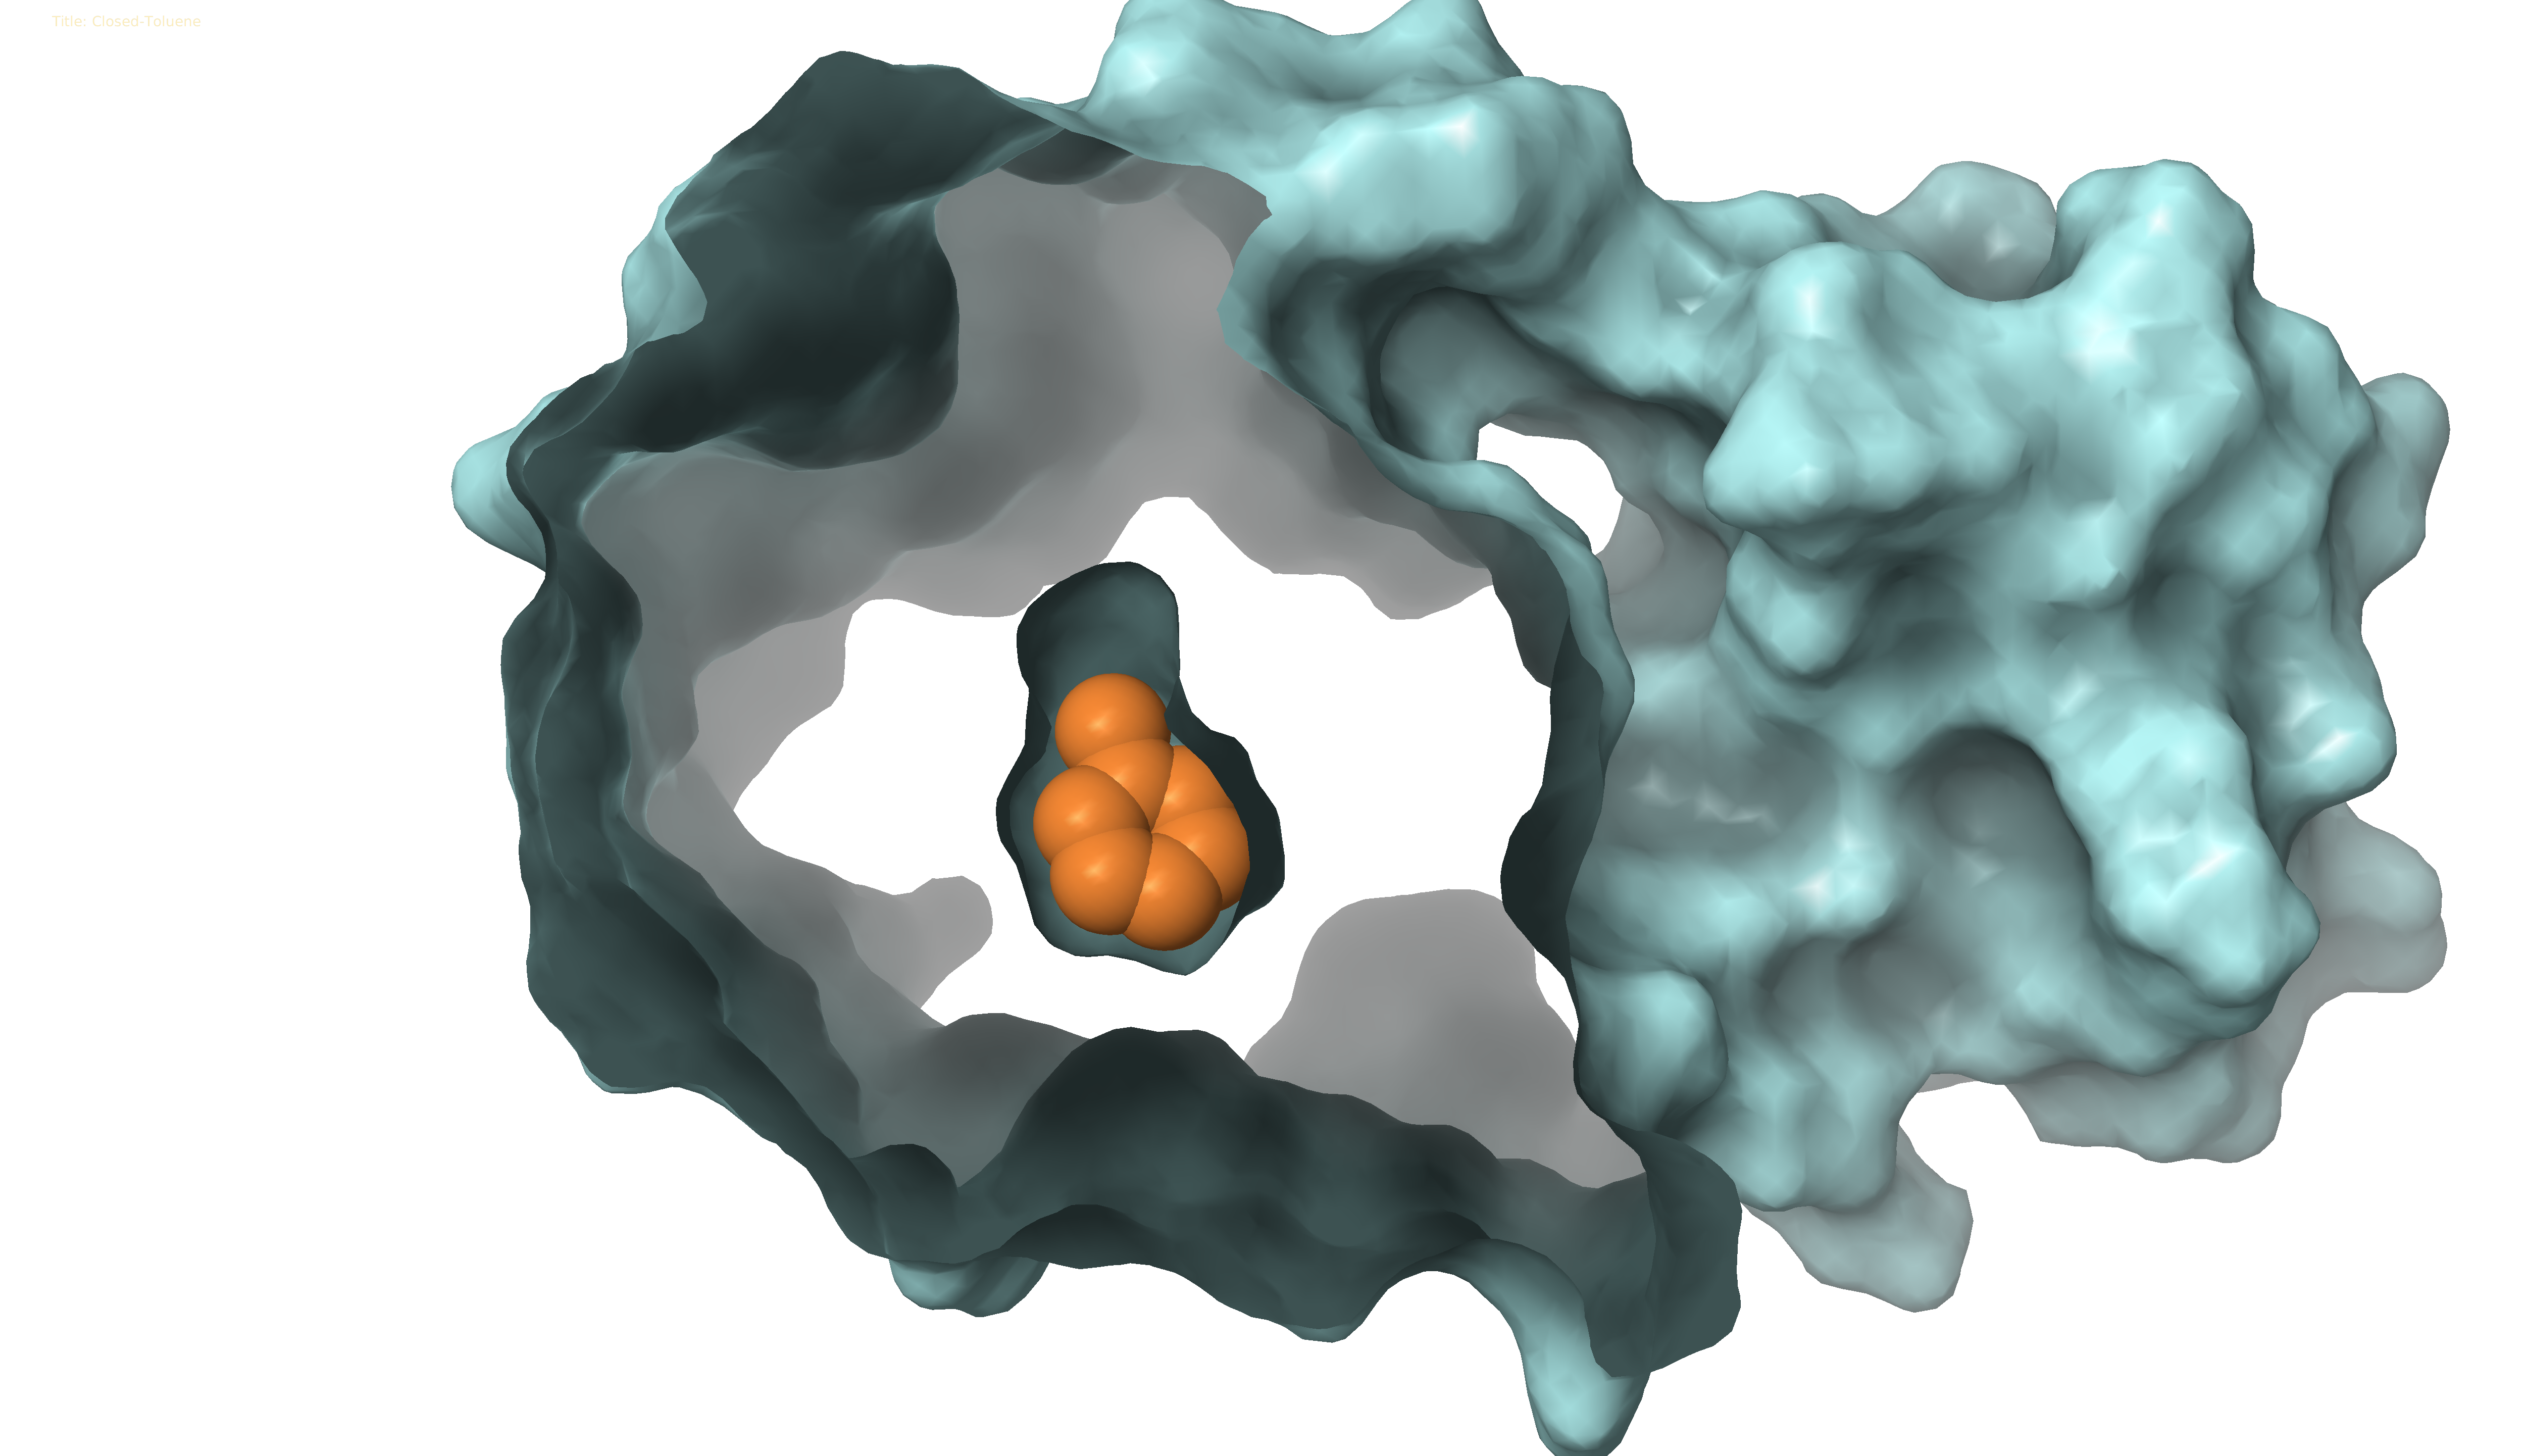
\includegraphics[trim={10cm 5cm 15cm 2cm}, clip, height=0.25\textheight]{Figures/Protein/closed_surface_trans.png}}
\end{subfigure}\hfill
\centering
\begin{subfigure}{0.30\textwidth}
  \centering
   \caption{Intermediate State}
   \label{fig:int_surface}
   \frame{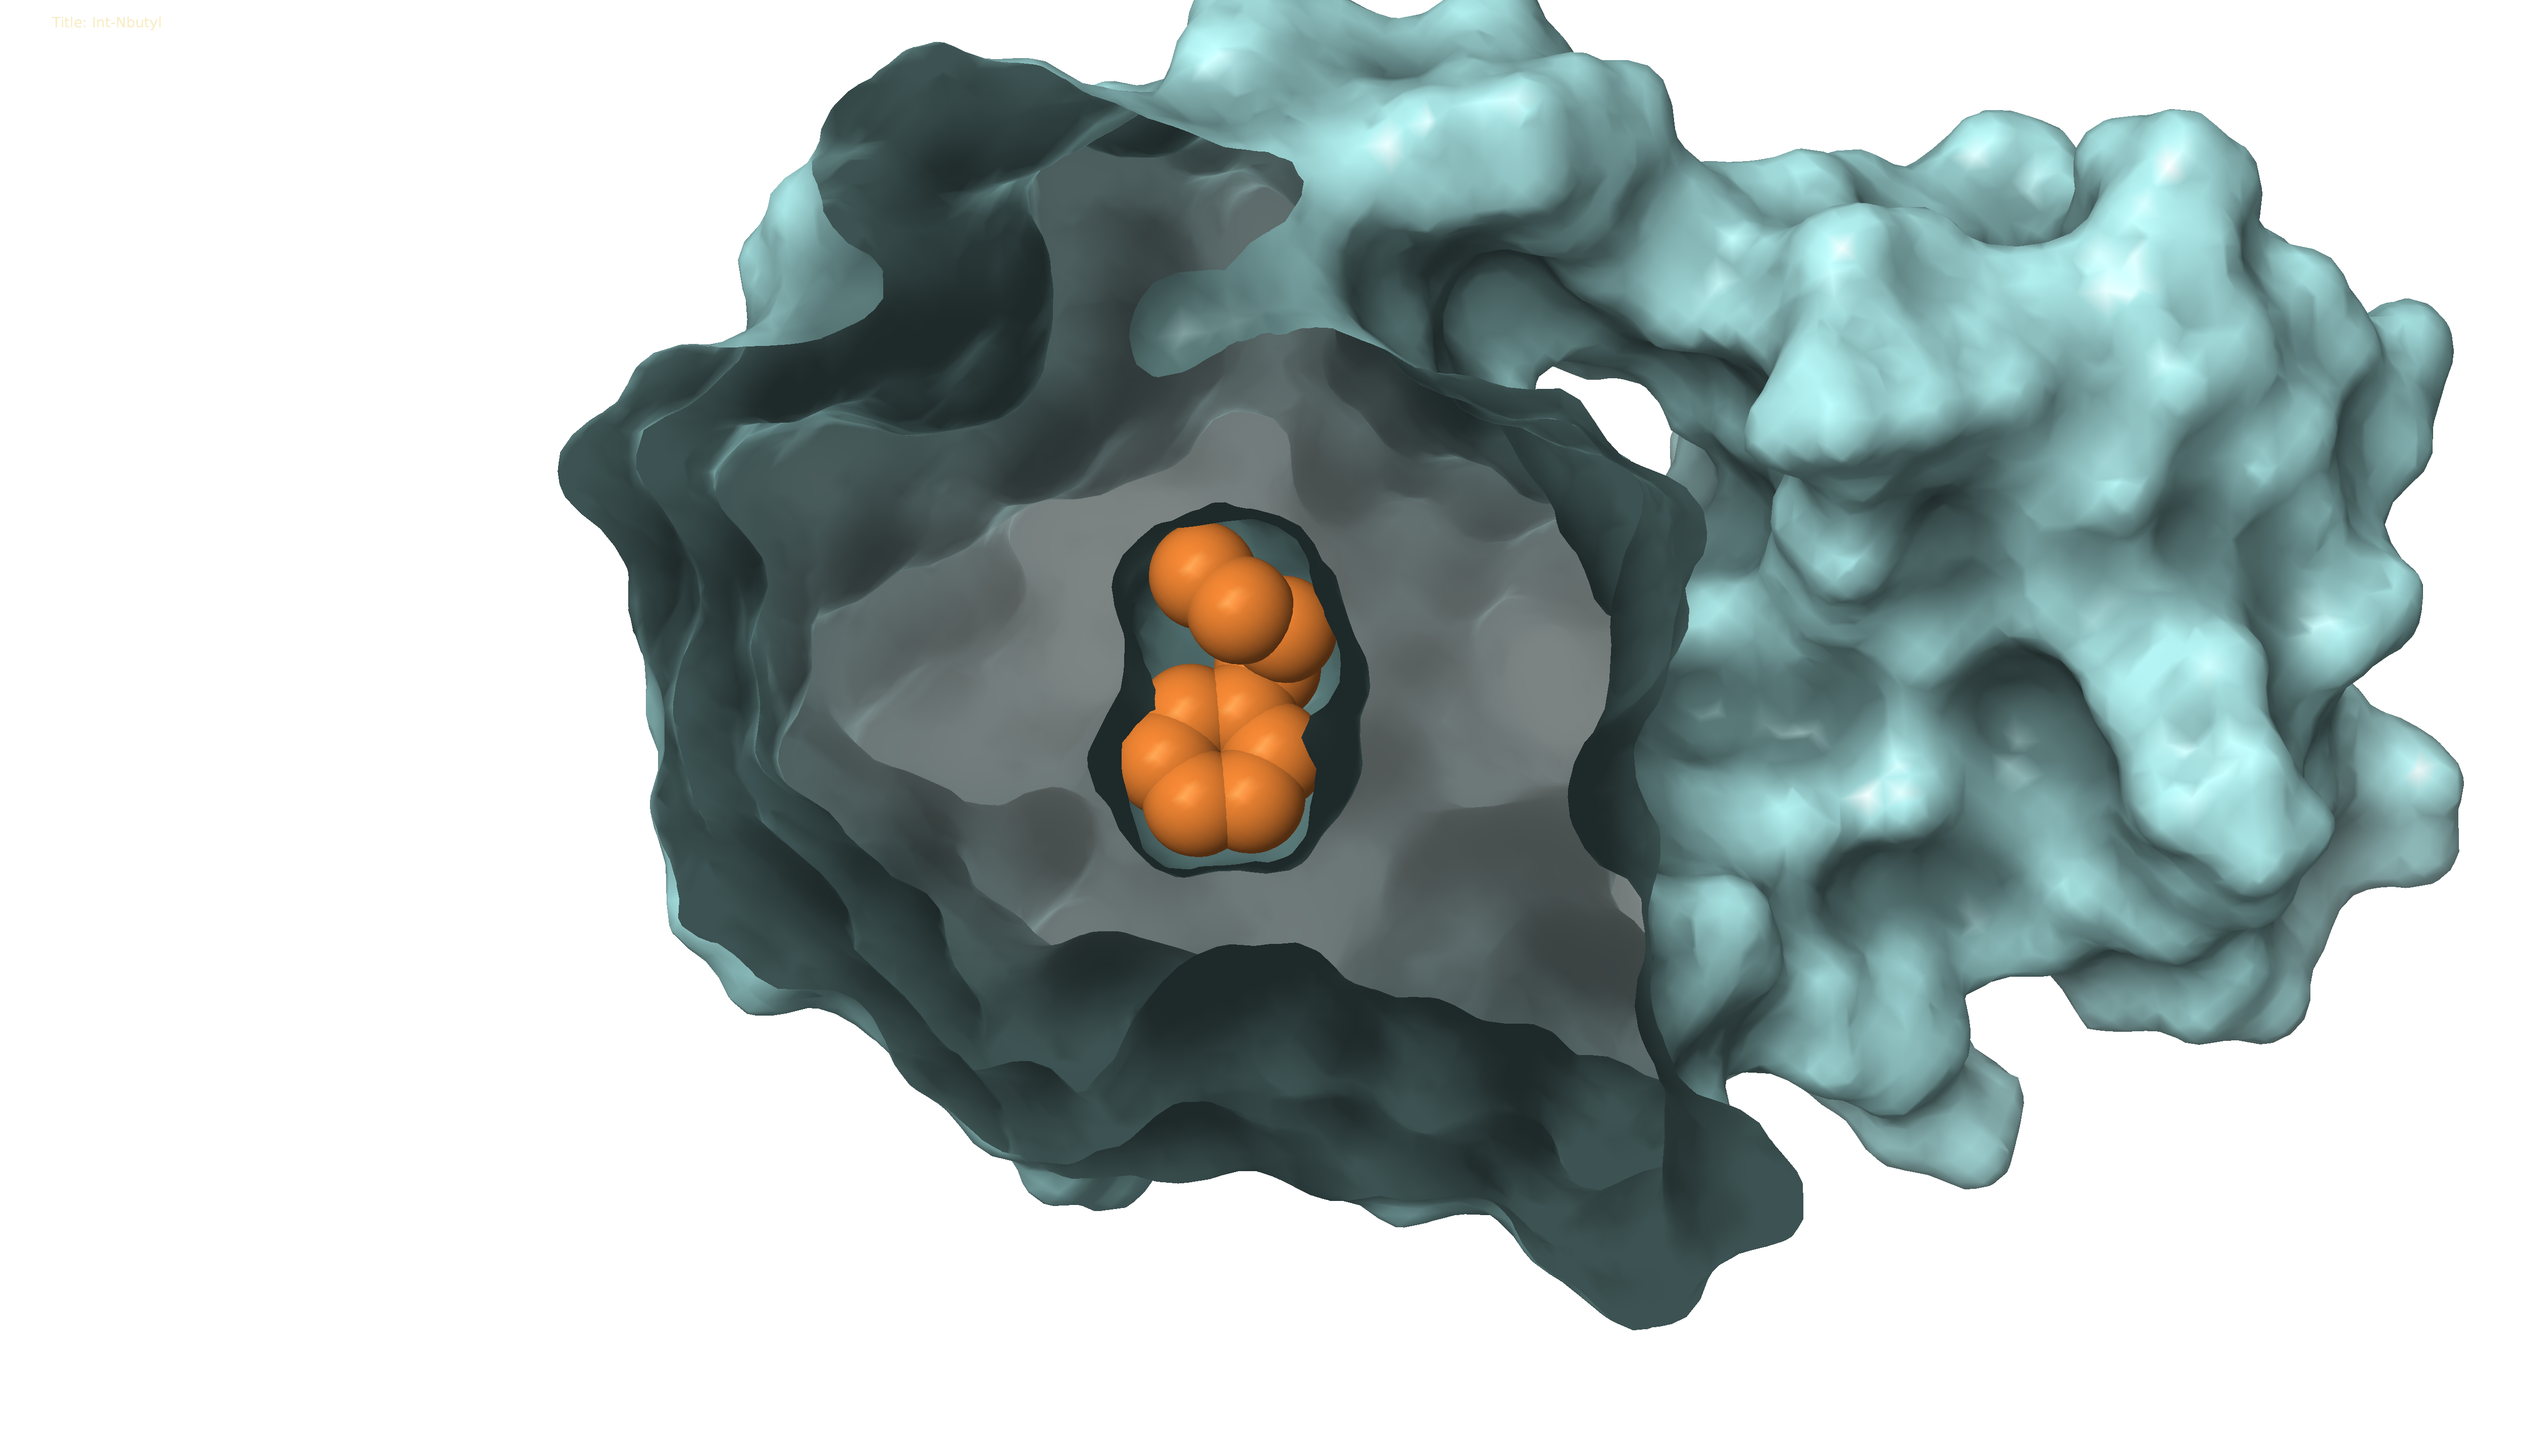
\includegraphics[trim={10cm 5cm 15cm 2cm}, clip, height=0.25\textheight]{Figures/Protein/int_surface_trans.png}}
\end{subfigure}\hfill
\centering
\begin{subfigure}{0.30\textwidth}
   \centering
   \caption{Open State}
   \label{fig:open_surface}
   \frame{\includegraphics[trim={5cm 5cm 15cm 2cm}, clip, width=\linewidth, height=0.25\textheight]{Figures/Protein/open_surface_trans.png}}
\end{subfigure}
\centering
\begin{subfigure}{0.75\textwidth}
   \centering
   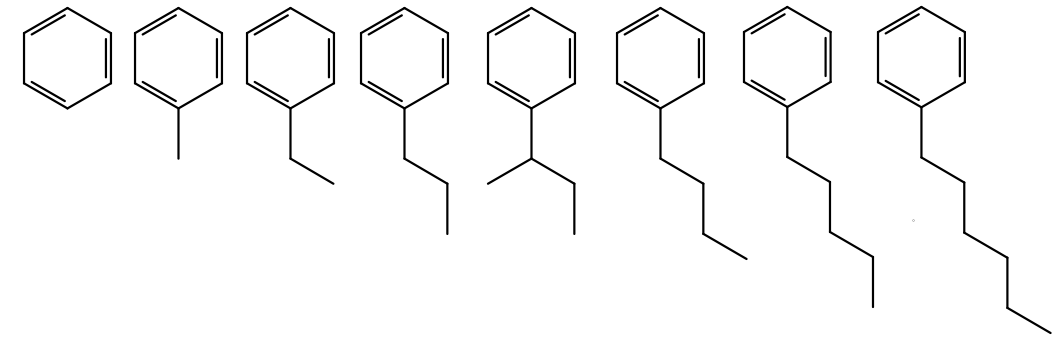
\includegraphics[clip, width=\textwidth, height=0.15\textheight]{Figures/Protein/ligand_set.png}
   \caption{Ligand Set}
   \label{fig:ligand_set}
\end{subfigure}\hfill
\caption{In Fig.\ref{fig:T4-L99A_protein} are overlaid cartoon representations of T4 lysozyme using the protein-ligand bound crystal structures of the toluene(4W53), butylbenzene(4W57), and hexylbenzene(4W59) complexes where the F-helix region is highlighted in yellow.
Fig.\ref{fig:T4-L99A_tube} illustrates a closer view of strictly the F-helix in the closed(purple), intermediate(cyan), and open(green) conformational states and their corresponding ligands as found in the crystal structure.
Below are the molecular surface representations of the binding cavity in the closed(\ref{fig:closed_surface}), intermediate(\ref{fig:int_surface}), and open(\ref{fig:open_surface}) states with the ligands represented in an orange space-filling model.
In Fig.\ref{fig:ligand_set} is the full series of congeneric ligands used in this study; their protein state occupancies can be found in Table~\ref{tbl:expdata}.
Images were created using Maestro\cite{Maestro}.}
\label{fig:T4-L99A}
\end{figure}

\begin{figure}[!ht]
\begin{subfigure}{\textwidth}
   \centering
   \caption{Selected residues in pREST}
   \label{fig:C2O}
   \frame{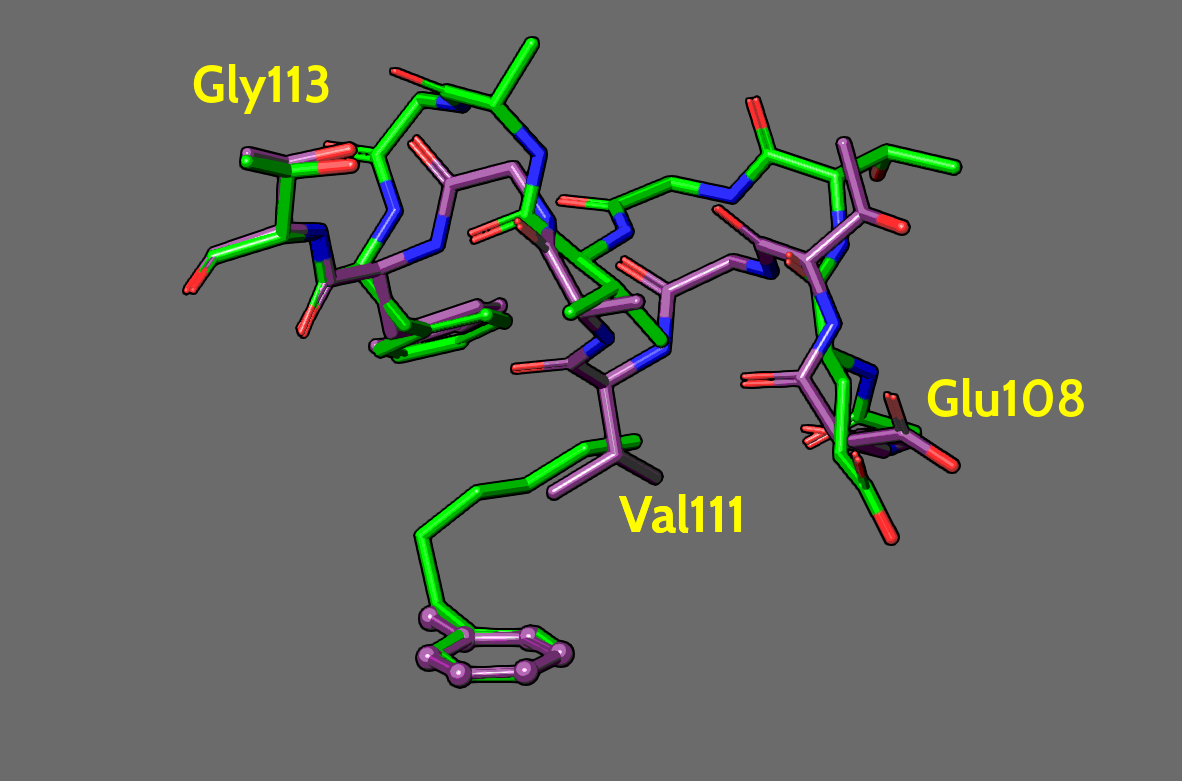
\includegraphics[trim={0cm 3cm 0cm 1cm}, clip, height=0.4\textheight]{Figures/Protein/C2O.png}}
\end{subfigure}\hfill
\centering
\begin{subfigure}{.45\textwidth}
  \centering
   \frame{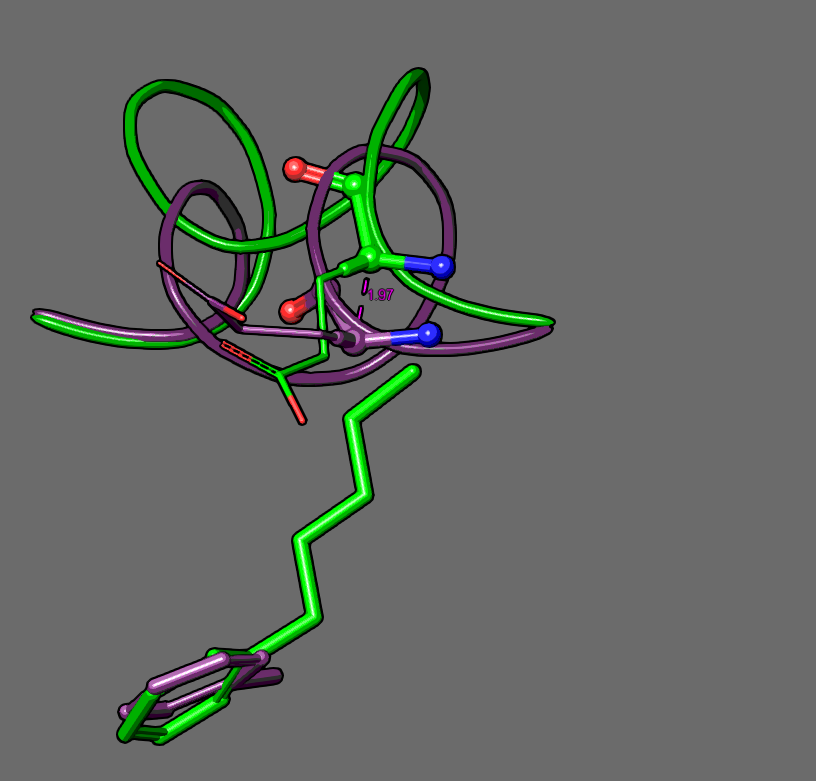
\includegraphics[trim={1cm 0cm 8cm 2cm}, clip, height=0.4\textheight]{Figures/Protein/Glu108-C2O.png}}
   \caption{Residue Glu108}
   \label{fig:Glu108-C2O}
\end{subfigure}\hfill
\begin{subfigure}{.55\textwidth}
   \centering
   \frame{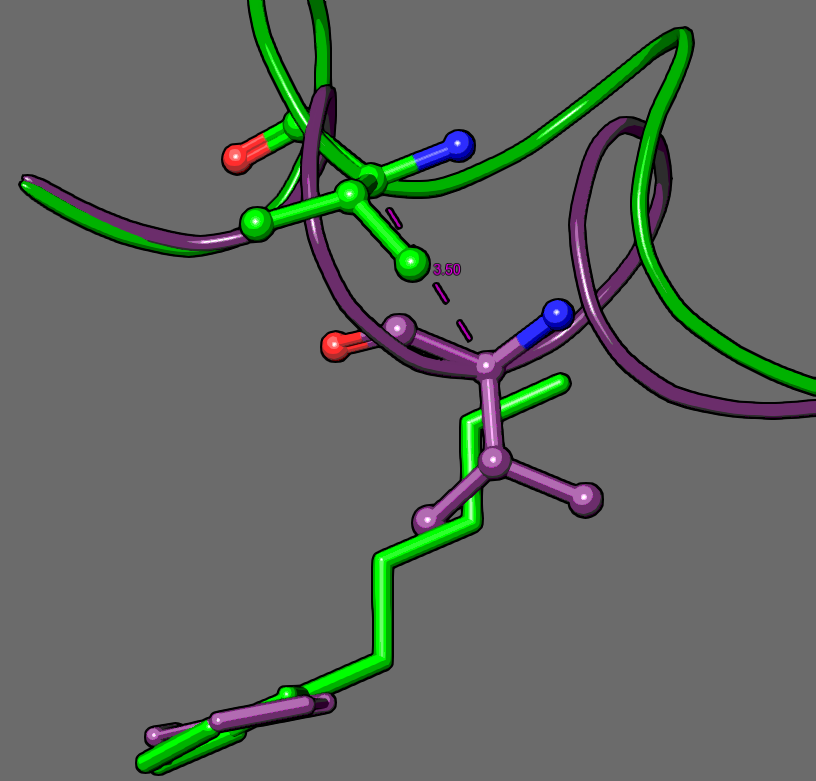
\includegraphics[trim={2cm 0cm 0cm 0cm}, clip, height=0.4\textheight]{Figures/Protein/Val111-C2O.png}}
   \caption{Residue Val111}
   \label{fig:Val111-C2O}
\end{subfigure}\hfill
\caption{Fig.~\ref{fig:C2O} highlights the 3 residues selected to be included into the REST region for `pREST' simulations. 
Fig.~\ref{fig:Glu108-C2O} and Fig.~\ref{fig:Val111-C2O} illustrates the motion of the $C_{\alpha}$'s during the transition between the protein closed and open states, where the $C_{\alpha}$ in Glu108 undergoes a motion of approximately 2\AA, while in Val11 the $C_{\alpha}$ move approximately 3.5\AA.}
\label{fig:pRESTresidues}
\end{figure}

\begin{figure}[!ht]
\begin{subfigure}{\textwidth}
   \centering
    \caption{Protein closed simulation}
   \label{fig:c_opls3_1/RMSD-replica11}
   \frame{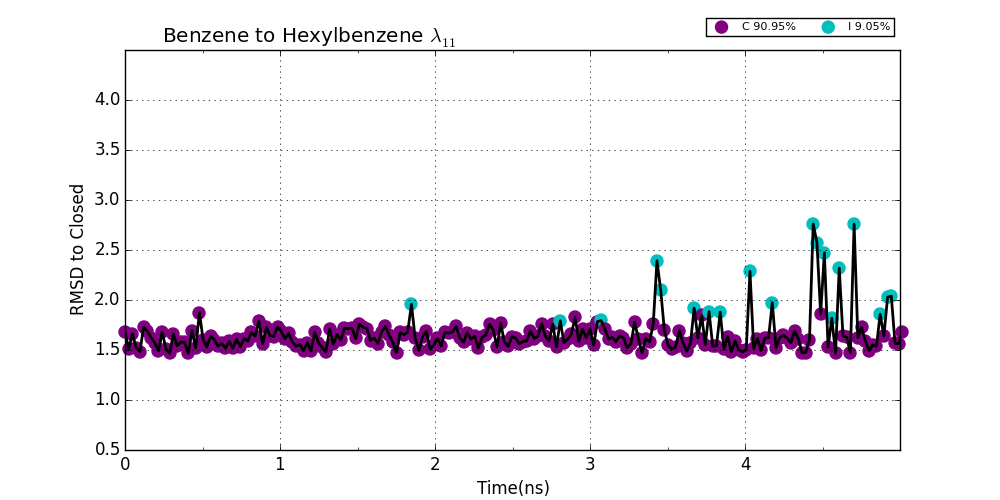
\includegraphics[trim={1.5cm 0 2cm 0.25cm}, clip, width=\linewidth, height=0.3\textheight]{Figures/RMSD-time/benzene-nhexylbenzene_C_default_rep11.png}}
\end{subfigure}
\centering
\begin{subfigure}{\textwidth}
  \centering
  \frame{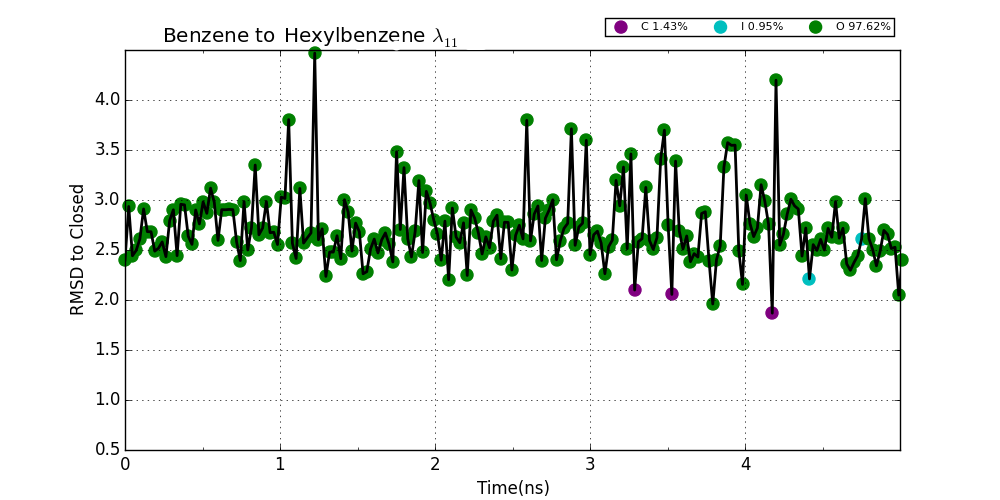
\includegraphics[trim={1.5cm 0 2cm 0.25cm}, clip, width=\linewidth, height=0.3\textheight]{Figures/RMSD-time/benzene-nhexylbenzene_O_default_rep11.png}}
  \caption{Protein open simulation}
  \label{fig:o_opls3_1/RMSD-replica11}
\end{subfigure}%
\caption{Plotted is the RMSD(\AA) relative to the closed helix conformation (black line), where each time point is colored according to the protein state of lowest RMSD to the trajectory. 
Here, using the default protocol in the transformation of benzene to hexylbenzene, RMSD/time plots correspond to the final end state of hexylbenzene ($\lambda_{11}$). 
Fig.~\ref{fig:c_opls3_1/RMSD-replica11} corresponds to the simulation that began from the protein closed state and Fig.~\ref{fig:o_opls3_1/RMSD-replica11} is from the simulation started from the protein open state. 
The legends indicate the percentage of sampling of each protein conformational state from the trajectory.}
\label{fig:benzene_to_n-hexyl}
\end{figure}

\begin{figure}[!ht]
\begin{subfigure}{.5\textwidth}
  \centering
  \caption{Default}
   \label{fig:c_opls3_1/colormap}
   \frame{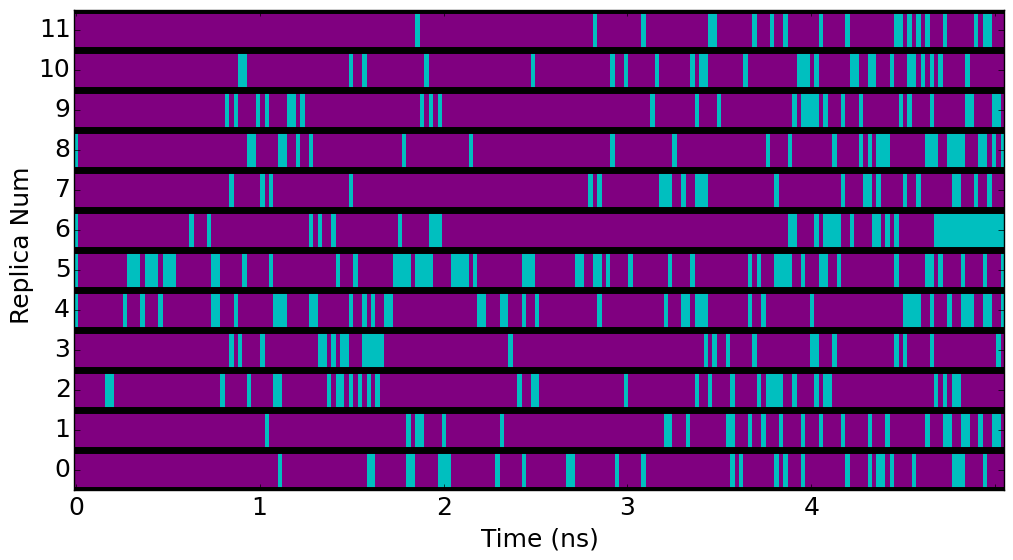
\includegraphics[width=\linewidth, height=0.3\textheight]{Figures/Colormap/benzene-nhexylbenzene_C_default.png}}
\end{subfigure}\hfill
\begin{subfigure}{.5\textwidth}
   \centering
    \caption{pREST}
   \label{fig:c_opls3_rest1_1/colormap}
   \frame{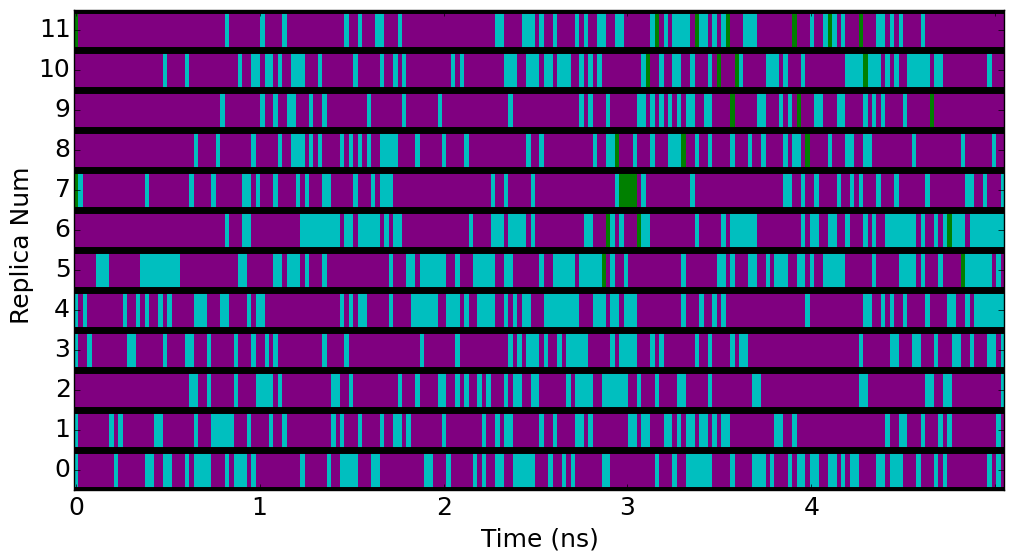
\includegraphics[width=\linewidth, height=0.3\textheight]{Figures/Colormap/benzene-nhexylbenzene_C_pREST.png}}

\end{subfigure}\hfill
\centering
\begin{subfigure}{\textwidth}
   \centering
   \frame{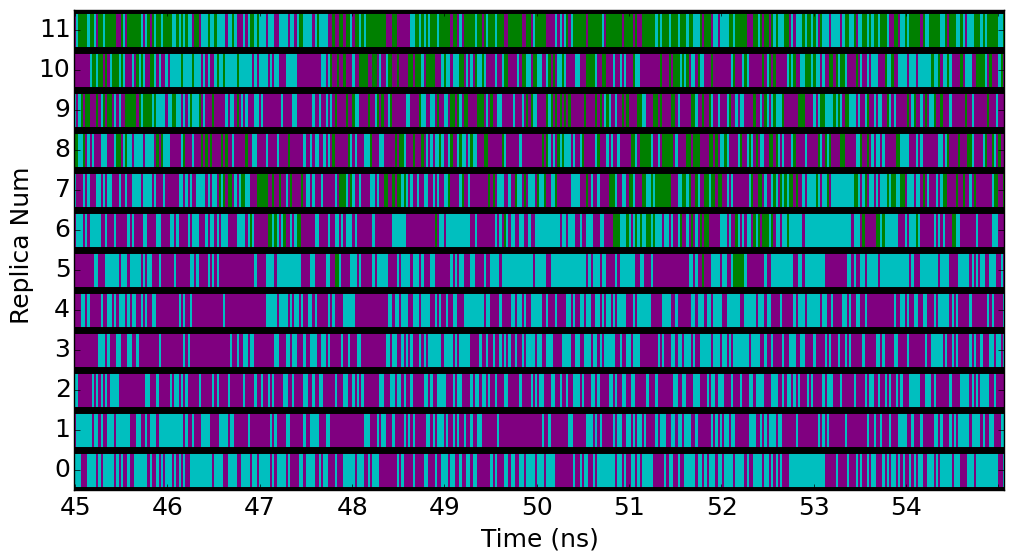
\includegraphics[clip, width=\linewidth, height=0.3\textheight]{Figures/Colormap/benzene-nhexylbenzene_C_pRESText.png}}
   \caption{pREST extended}
   \label{fig:c_opls3_rest1_1/cmap-45-55ns}
\end{subfigure}\hfill
\caption{Color maps of simulations starting from the protein closed state for the benzene to hexylbenzene alchemical transformation. 
Lines at every frame are colored accordingly to the protein state of lowest RMSD (purple-closed, cyan-intermediate, green-open). 
Fig.~\ref{fig:c_opls3_1/colormap} corresponds to simulations using the default protocol. Fig.~\ref{fig:c_opls3_rest1_1/colormap} represents simulations using the modified REST region protocol (pREST). Fig.~\ref{fig:c_opls3_rest1_1/cmap-45-55ns} illustrates the enhancement in protein conformational sampling through extending the pREST simulation time up to 55ns. 
}
\label{fig:benzene_to_n-hexyl_colormap}
\end{figure}

\begin{figure}[!ht]
\centering
\begin{subfigure}{.5\textwidth}
  \centering
    \caption{Closed-Open: Default}
   \label{fig:C2O_xyplot}
   \frame{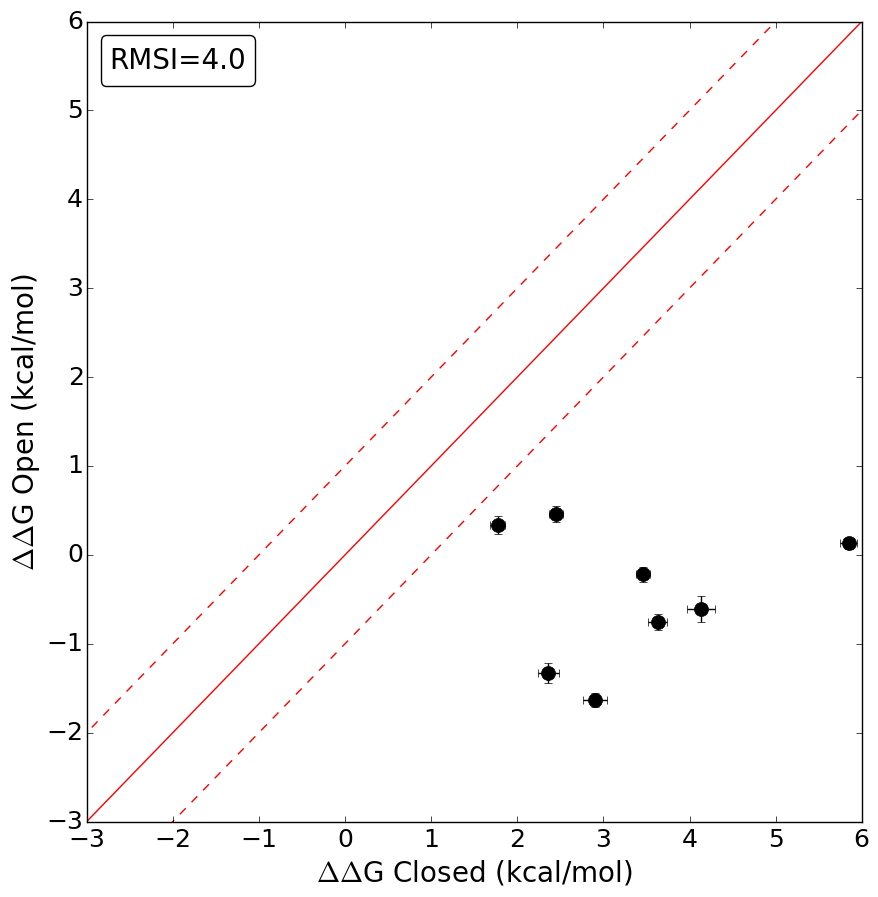
\includegraphics[width=\linewidth, height=0.3\textheight]{Figures/XYplot/C2O_xyplot.png}}
\end{subfigure}\hfill
\begin{subfigure}{.5\textwidth}
   \centering
  \caption{Closed-Open: pREST}
   \label{fig:C2O_xyplot_pREST}
   \frame{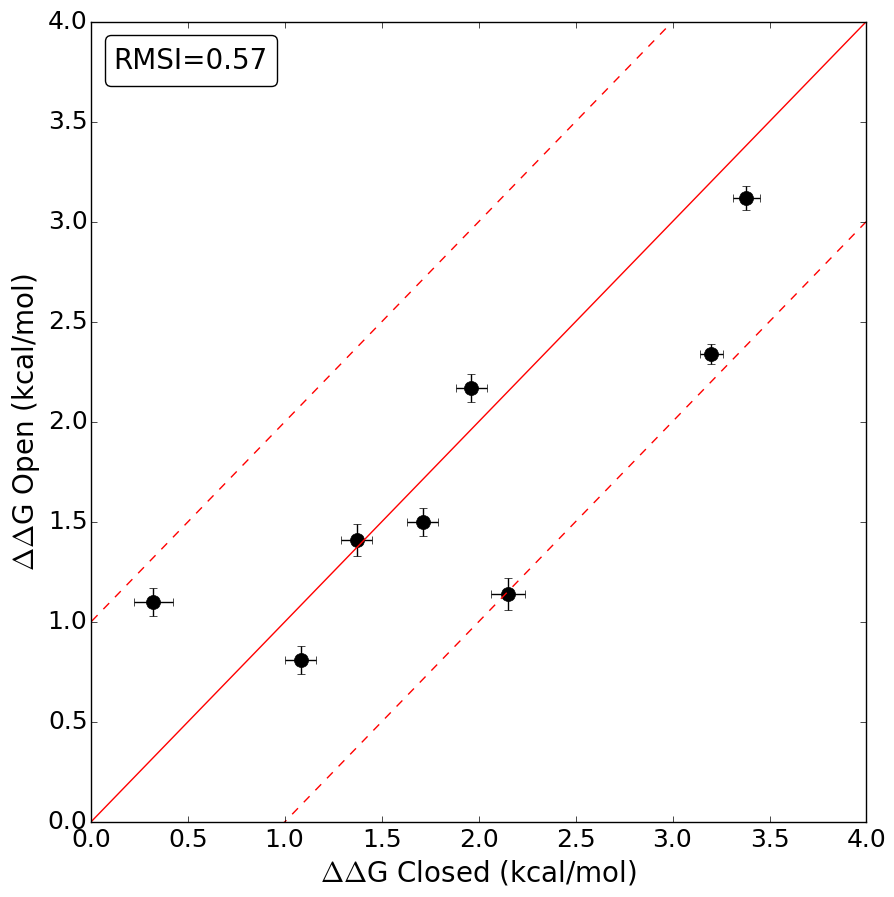
\includegraphics[width=\linewidth, height=0.3\textheight]{Figures/XYplot/C2O_pREST_xyplot.png}}
\end{subfigure}\hfill
\centering
\begin{subfigure}{.5\textwidth}
  \centering
   \frame{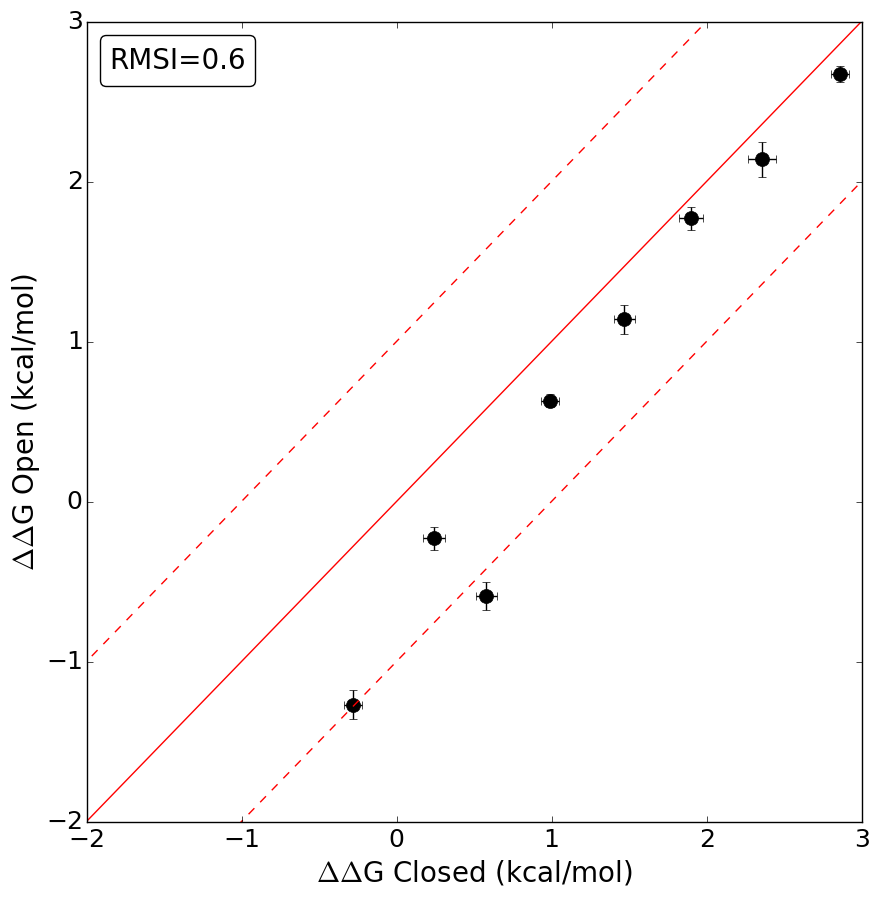
\includegraphics[width=\linewidth, height=0.3\textheight]{Figures/XYplot/C2I_xyplot.png}}
   \caption{Closed-Intermediate: Default}
   \label{fig:C2I_xyplot}
\end{subfigure}\hfill
\begin{subfigure}{.5\textwidth}
   \centering
   \frame{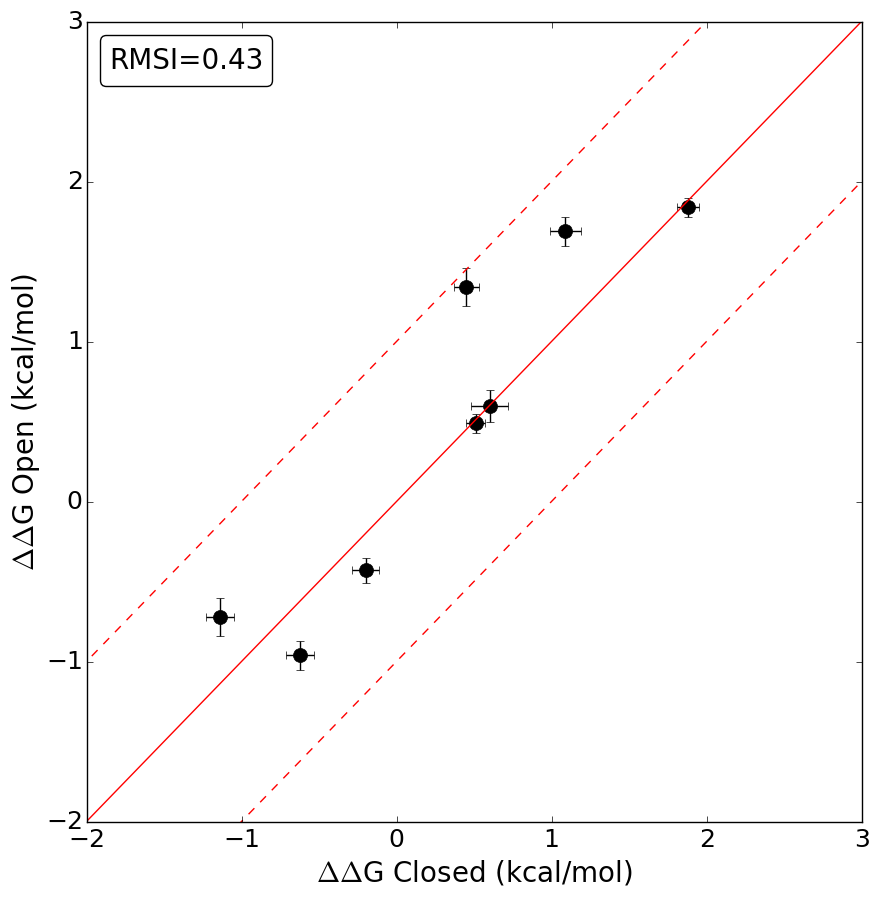
\includegraphics[width=\linewidth, height=0.3\textheight]{Figures/XYplot/C2I_pREST_xyplot.png}}
   \caption{Closed-Intermediate: pREST}
   \label{fig:C2I_xyplot_pREST}
\end{subfigure}\hfill
\caption{$\Delta\Delta G_{calc}$ from MD simulations beginning from the protein closed versus open state. 
Fig.~\ref{fig:C2O_xyplot} plots relative free energies obtained using the default protocol from the `closed-open' alchemical transformations set, yielding a RMSI of 4.0 kcal/mol. 
Fig.~\ref{fig:C2O_xyplot_pREST} are the final computed free energies with simulations carried out to 55ns using pREST, giving RMSI of 0.57 kcal/mol. 
Fig.~\ref{fig:C2I_xyplot} plots relative free energies from the `closed-intermediate' set using the default protocol which gives an RMSI of 0.6 kcal/mol. 
Fig.~\ref{fig:C2I_xyplot_pREST} are free energies with simulations carried out up to 25ns using pREST, giving RMSI of 0.43 kcal/mol. 
Numerical data for each plot can be found in Tables~S\ref{tbl:C-I}, S\ref{tbl:C-I_pRESText}, \ref{tbl:C-O}, and SS\ref{tbl:C-O_pREST-40-55ns}.
}
\label{fig:conf-xyplots}
\end{figure}


\begin{figure}[!ht]
\centering
\begin{subfigure}{.5\textwidth}
  \centering
     \caption{Default}
   \label{fig:exp_xyplot}
   \frame{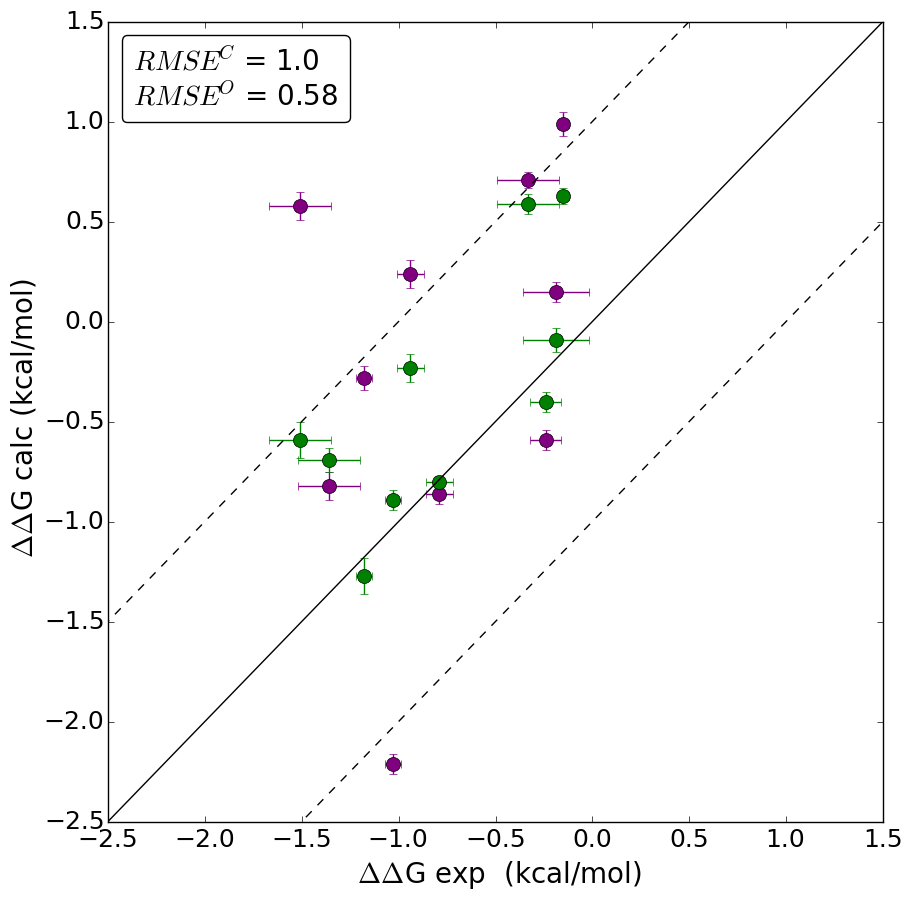
\includegraphics[width=\linewidth, height=0.3\textheight]{Figures/XYplot/exp_xyplot.png}}
\end{subfigure}\hfill
\begin{subfigure}{.5\textwidth}
   \centering
      \caption{pREST}
   \label{fig:exp_xyplot_pREST}
   \frame{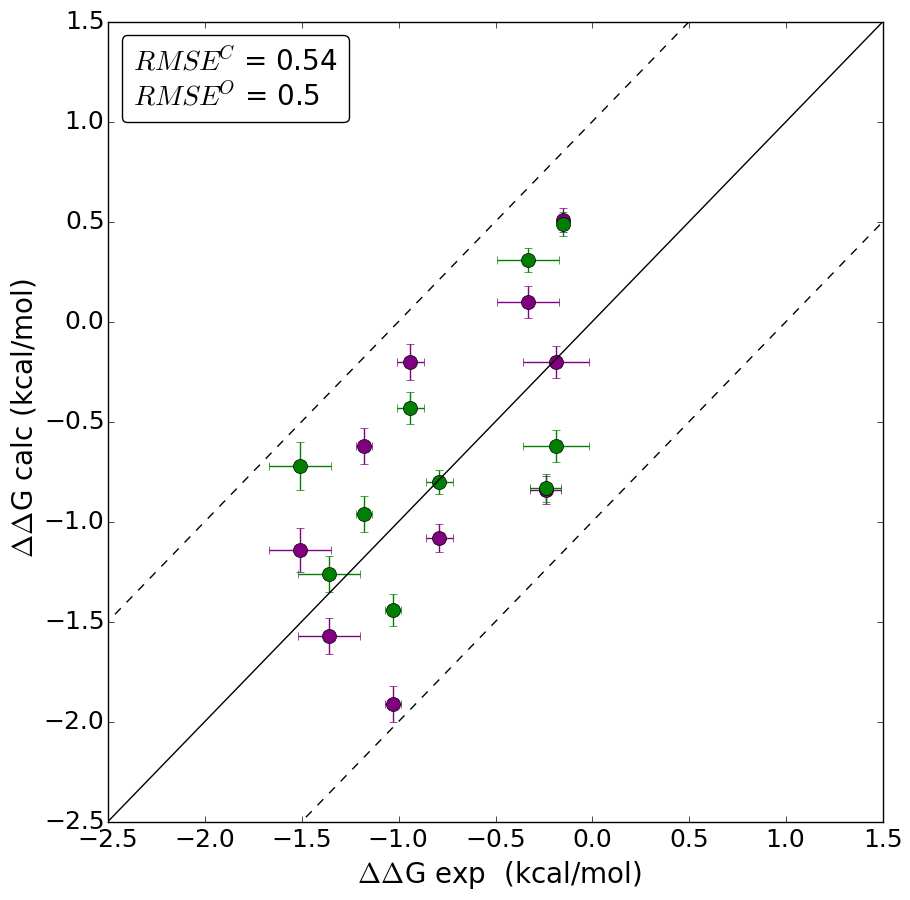
\includegraphics[width=\linewidth, height=0.3\textheight]{Figures/XYplot/exp_pREST_xyplot.png}}
\end{subfigure}\hfill
\caption{$\Delta\Delta G_{calc}$ from MD simulations beginning from the protein closed (purple) and open (green) state compared against $\Delta\Delta G_{exp}$. 
Fig.~\ref{fig:exp_xyplot} plots free energies obtained using the default protocol which gives a 1.0 kcal/mol and 0.58 kcal/mol RMSE for protein closed and open simulations, respectively.
Total RMSI using the default protocol is 0.68 kcal/mol. 
Fig.~\ref{fig:exp_xyplot_pREST} plots the final free energies after applying pREST, yielding an RMSE of 0.54 for protein closed and 0.50 kcal/mol for protein closed simulations.
Total RMSI using the pREST protocol is 0.31 kcal/mol.
Numerical data for each plot can be found in Tables~S\ref{tbl:exp_set} and S\ref{tbl:exp_pREST_set}.
} 
\label{fig:exp-xyplots}
\end{figure}


\begin{figure}[!ht]
\begin{subfigure}{\textwidth}
   \centering
    \caption{Protein closed simulation}
   \label{fig:c_exp_opls3_11/RMSD-replica11}
   \frame{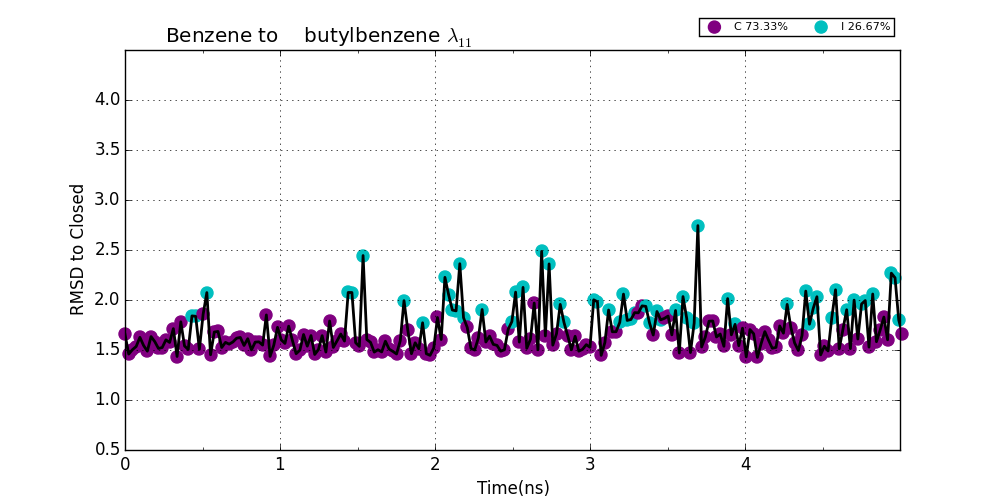
\includegraphics[trim={1.5cm 0 2cm 0.25cm}, clip, width=\linewidth, height=0.3\textheight]{Figures/RMSD-time/benzene-nbutylbenzene_C_default_rep11.png}}
\end{subfigure}
\centering
\begin{subfigure}{\textwidth}
  \centering
   \frame{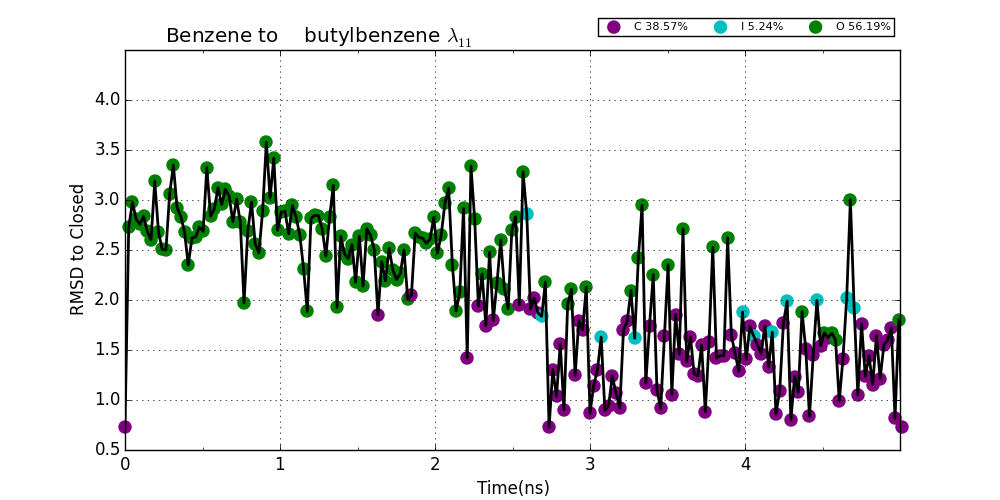
\includegraphics[trim={1.5cm 0 2cm 0.25cm}, clip, width=\linewidth, height=0.3\textheight]{Figures/RMSD-time/benzene-nbutylbenzene_O_default_rep11.png}}
   \caption{Protein open simulation}
   \label{fig:o_exp_opls3_24/RMSD-replica11}
\end{subfigure}%
\caption{RMSD/time plots correspond to the final end state of butylbenzene ($\lambda_{11}$) while using the default protocol for transformation of benzene to butylbenzene. 
Fig.~\ref{fig:c_exp_opls3_11/RMSD-replica11} and Fig.~\ref{fig:o_exp_opls3_24/RMSD-replica11} 
correspond to simulations that were started from the protein closed or open state, respectively. 
The legends indicate the percentage of sampling of each protein conformational state from the trajectory.
}
\label{fig:benzene_to_n-butyl}
\end{figure}

\begin{figure}[!ht]
\begin{subfigure}{\textwidth}
   \centering
    \caption{Protein closed simulation, pREST}
   \label{fig:c_opls3_rest1_1/RMSD-replica11}
   \frame{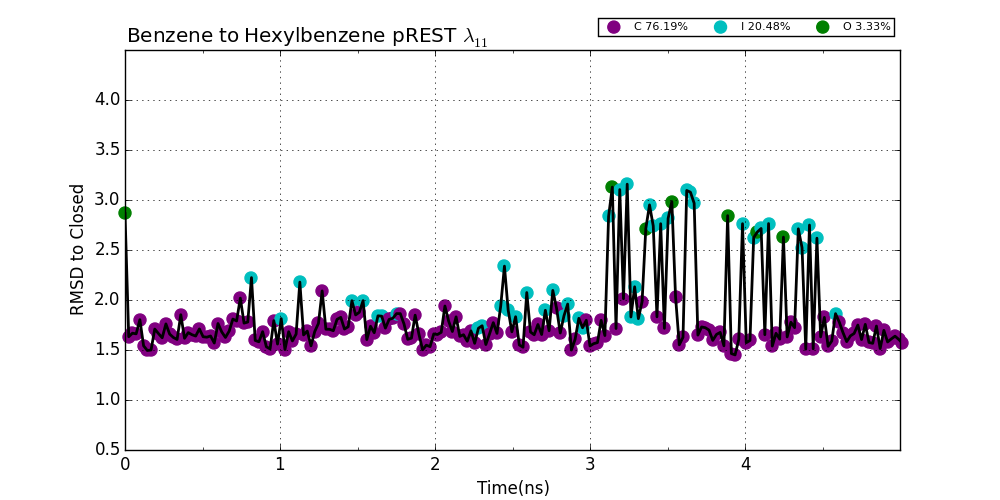
\includegraphics[trim={1.5cm 0 2cm 0.25cm}, clip, width=\linewidth, height=0.3\textheight]{Figures/RMSD-time/benzene-nhexylbenzene_C_pREST_rep11.png}}
\end{subfigure}
\centering
\begin{subfigure}{\textwidth}
  \centering
   \frame{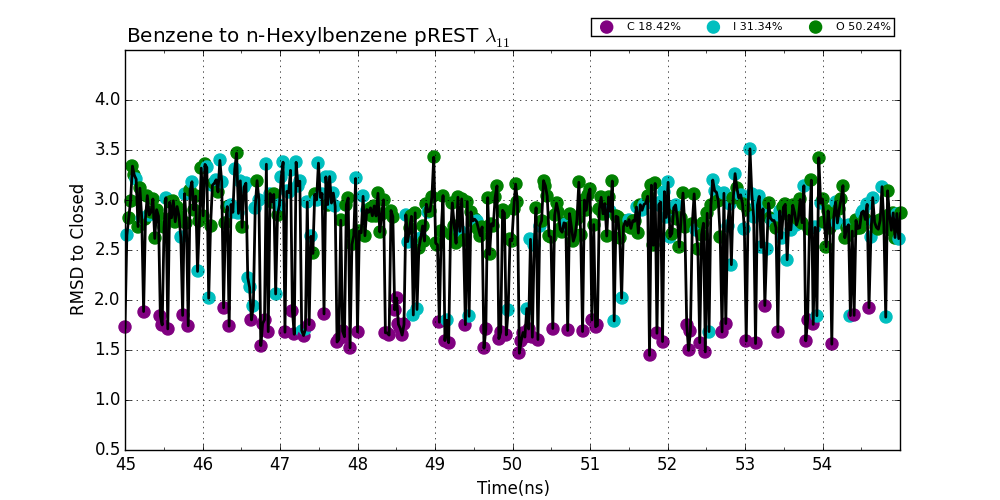
\includegraphics[trim={1.5cm 0 2cm 0.25cm}, clip, width=\linewidth, height=0.3\textheight]{Figures/RMSD-time/benzene-nhexylbenzene_C_pRESText_rep11.png}}
   \caption{Protein closed simulation, pREST extended}
   \label{fig:c_opls3_rest1_1/45-55ns/RMSD-replica11}
\end{subfigure}%
\caption{Using the modified REST region (pREST) in the transformation of benzene to hexylbenzene, we plot the RMSD/time corresponding to the hexylbenzene state ($\lambda_{11}$) with the simulation starting from protein closed for the first 5ns (Fig.~\ref{fig:c_opls3_rest1_1/RMSD-replica11}) and the final 10ns from an extended run up to 55ns (Fig.~\ref{fig:c_opls3_rest1_1/45-55ns/RMSD-replica11}).}
\label{fig:benzene_to_n-hexyl_pREST}
\end{figure}





